\documentclass[12pt]{article}
\usepackage[utf8]{inputenc}
\usepackage{graphicx}
\usepackage{amssymb}

\title{Introduction to writing documents in Latex}
\author{Jorge Mario Laveaga Vergara}
\date{07/12/2020}

\begin{document}
	\maketitle
	
	\section{Before writing your document}
		\subsection{TeX vs LaTeX}
		{TeX is a typesetting system which was designed and mostly written by Donald Knuth, designed with the goals of allowing anyone to produce high quality books adn to provide a system that would give exactly the same results on all computers. TeX reached it's first objective by being a free software. LaTeX is a generalised set of macros for TeX. It's basically an easier and less technical version of TeX.}\par
		\subsection{Introduction to what LaTeX is.}
			{According to \textit{The Latex Project} website, LaTeX (Pronounced "Lah-tech") is a document preperation system for high-quality typesetting.  \cite{latexOfficial}(2020). LaTeX is available as free software.}\par
			{More specifically, LaTeX is a software system for document preparation. It utilizes plain text (unlike formatted text from word processors like Microsoft Word). LaTeX utilizes markup tagging (Basically it means the LaTeX code you don't see when you look at the document) for the general structure of a document, to stylise text throughout a document and to add citations and cross-references.}\par \cite{latexWikipedia}
			
			{LaTeX is not like word, where you have to "design" the document. LaTeX allows you to just focus on the content of your document, and leave the document design to document designers.}\par
			{Latex has various features, and as stated before, it has high-quality typesetting, which just means it allows:}\par 
			\begin{itemize}
				\item[1.]{Typesetting Journal articles, technical reports, books, and slide presentations.}\par
				\item[2.] {Control over large documents containing sectioning, cross-references, tables and figures.}\par
				\item[3.]{Typesetting of complex mathematical formulas}\par
				\item[4.]{Advanced typesetting with AMS-LaTeX}\par
				\item[5.]{Automatic generation of bibliographis and indexes}\par
				\item[6.]{Automatic generation of bibiliographis and indexes}\par
				\item[7.]{Multi-lingual typesetting}\par
				\item[8.]{Inclusion of artwork and process or spot color}\par
				\item[9.]{Using PostScript or Metafont fonts.}\par
			\end{itemize}
	\section{Basic structure of a LaTeX document}
		{Usually you start the document in an editor, such as Texworks or TexMaker, which will give you a space from where to write your LaTeX instructions. Usually the basic set of instructions looks like the following: }\par
		\begin{center}
			\begin{figure}
				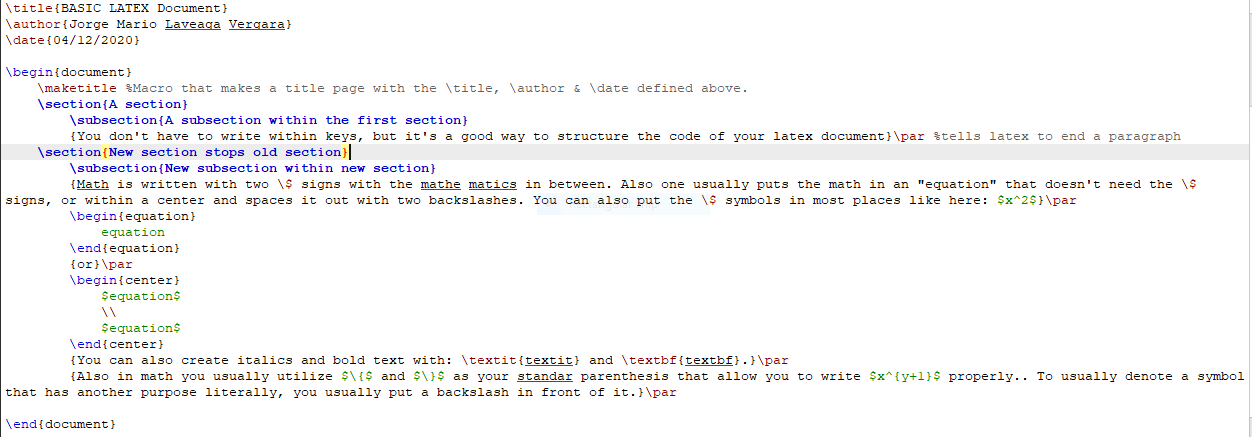
\includegraphics[scale=0.3]{ExampleLatexPicture}
				\includegraphics[scale=0.3]{BasicLatexStructure}
			\end{figure}
		\end{center}
	\section{How this document is written}
\end{document}
\begin{thebibliography
	\bibitem{latexOfficial}
	{The Latex Project. (2020) Electronic Website. Recovered from:"https://www.latex-project.org/"}\par
	\bibitem{latexWikipedia}
	{LaTeX. (2020) Wikipedia. Recovered from:"https://en.wikipedia.org/wiki/LaTeX"}\par
\end{thebibiliography}